\documentclass[conference]{IEEEtran}
\IEEEoverridecommandlockouts
% The preceding line is only needed to identify funding in the first footnote. If that is unneeded, please comment it out.
\usepackage{cite}
\usepackage{amsmath,amssymb,amsfonts}
\usepackage{algorithmic}
\usepackage{booktabs}
\usepackage{float}
\usepackage{graphicx}
% \usepackage{longtable}
\usepackage{textcomp}
\usepackage{xcolor}
\def\BibTeX{{\rm B\kern-.05em{\sc i\kern-.025em b}\kern-.08em
    T\kern-.1667em\lower.7ex\hbox{E}\kern-.125emX}}
\begin{document}

\title{Simple Driving-Skill Evaluation System\\
\thanks{Identify applicable funding agency here. If none, delete this.}
}

\author{\IEEEauthorblockN{Yuan-Pu Hsu}
\IEEEauthorblockA{\textit{University of California, Riverside} \\
yhsu018@ucr.edu}
\and
\IEEEauthorblockN{Tianxiang Sun}
\IEEEauthorblockA{\textit{University of California, Riverside} \\
tsun024@ucr.edu}
}

\maketitle

\begin{abstract}
In this project, we implemented a simple driving-skill evaluation system, which can be put behind the windscreen of the car and recognizing patterns showing up on the road. By  comparing the pattern we got with the speed of the car, we can evaluate the driving skill of the driver. We built our own iOS application, constructed multiple Convolutional Neural Network (CNN) models to recognize traffic signs and traffic lights and achieving 99.8\% test accuracy for recognizing images taken in South California. The application can connect with different platforms, like Google Compute Engine (GCE) and local terminal (PC) via PHP protocol. In the end, we found that there existed a performance trade off between the accuracy and the time latency between different platform.
\end{abstract}

\begin{IEEEkeywords}
Driving-skill evalution, Convolutional Neural Network (CNN),  Google Compute Engine, PHP
\end{IEEEkeywords}

\section{Introduction}
% Driving has became a indispensable part of American's daily life for decades. It gives us a lot of convenience. Meanwhile, unskillful driving could cause serious damage, not only for drivers but also for the society. Therefore, a driving skill evaluation system would be a  nowadays. 
Nowadays, over 90\% of families in the United States at least have one vehicle. Driving has already been a big portion of American's daily life for decades. Therefore, we want to make a simple system to evaluate the driving skill of drivers after finish a tour, and the only thing needed is a smart phone. We believe it could help drivers to evaluate their driving skill and improve their skill to some extent. Furthermore, insurance company can also take advantage of this system to evaluate the credit of their clients by using their scores, while those who has higher scores, which means better driving skill could be benefit with lower insurance payment.

When it comes to details, firstly we build an application on our mobile device (in our case, iPhone6s) and use it to implement our system on. The user would be asked to put the phone behind the windscreen, and the application would automatically capture images of front view to recognize different kinds of patterns on the road. In our project, the recognized pattern has been restricted to traffic signs and traffic light. Additionally, in order to recognize patterns, we proposed a 6-layers CNN network, which consisted by 6 convolutional layers, 3 max-pooling layers, 3 drop-out layers and a fully connected layer with softmax. The test accuracy of our model for GTBSRB is 96.4\%.  Beside, by using Lisa dataset, test accuracy of traffic signs is 99.8\% and it is 99.5\% for traffic light. What is more, we implement our model on three different kinds platforms, iphone, google cloud and local terminal. We calculate the data transfer time, CNN model running time and server running time (if they have)for those three platforms, respectively. The result


The contribution of our project is shown as follows: 

\begin{itemize}
  \item We design our own iOS application by Swift deploying on iOS 11.2. In addition, we are able to measure the speed and acceleration, and compare with the recognized traffic sign and traffic light from road image in nearly real-time 
  \item We propose and construct our own CNN architecture which is a 6-layers CNN with 3 max-pooling layers, 3 drop-out layers and 1 fully-connected layer with softmax to conclude the results. The model is trained by using German Traffic Sign Recognition Benchmark (GTSRB) and LISA dataset for different kinds of scenarios.
%   \item We evaluate the performance of our model. The result shows that our model can reach at least 96.4\% test accuracy with GTRSRB dataset, 99.5\% test accuracy for traffic lights and 99.8\% for traffic signs with LISA dataset.
  \item We implement three platforms to run our model on: mobile device, GCE and PC. In order to implement our platform, evaluations had been done to decide which GPU we can used in GCE. Besides, we use those three platforms to test the model we build.
  \item  We use PHP protocol to enable our application to communicate with other platforms. It could upload images captured by the application to other platforms. After the server received the test image, they could run the CNN model to determine the pattern. Meanwhile, we evaluated the data-transfer time, running time with different Internet connection and on different platforms.
\end{itemize}

\section{Background and Related Work}

\subsection{Background}

\subsubsection{Convolutional Neural Network}

\

\noindent
Convolutional Neural Network(CNN) is a important, widely-used model in machine learning. It is a class of deep, feed-forward artificial neural networks, most commonly applied to analyzing visual imagery. The following is brief introduction about the layer architecture we chose: 
\begin{itemize}
\item \textbf{Convolutional layer} apply a convolution operation to the input and pass it to the output. By doing convolution between original image and filters, more detailed information are gotten and a feature map has been created.
\item\textbf{Max-pooling layer} is used to reshape the image by using the maximum value from each of the cluster of neurons at the prior layer.
\item\textbf{Drop-out layer} is a regularization technique to drop out some units in a neural network to reduce over-fit in neural network.
\item\textbf{Fully-connected layer with softmax} is used to flatten the result we gotten before. What is more, softmax can be using as the classifier to get the classification of the network.
\end{itemize}


\subsubsection{Tensorflow and Keras}

\noindent
\begin{itemize}
\item\textbf{Tensorflow} is an open source soeftware libaray for high performance numerical computation. Its flexible architecture allows easy deployment of computation acrosss a variety of platforms, and from desktop to clusters of serves to mobile and edge devices. In machine learning and deep learning, it does strong support and has been widely used.

\item\textbf{Keras} is a high-level neural networks API, written in Python and capable running on top of Tensorflow, CNTK, or Theano. It is much easier to deploy our own neural network by using it. Furthermore, it can decrease the running time significantly, which makes fast experimentation enable. 
\end{itemize}


\subsection{Related Work}

Before we began our work,we had been inspired by the work of Kang,Y.P. et al. [1]. In their paper, they did partitions for the neural network and running various parts on different platforms. Besides, Kang and his team evaluated the latency and energy consumption of their new system, which showed that their new system can achieve up to $40.7 \times$ latency speed-up, reduce mobile energy consumption by up to $94.7 \%$, and improve data-center throughput by up to $6.7 \times$. Additionally, we also got some inspired by the work of Shustanov, A. et al. [2] and Habibi Aghdam, H., et al [3]. while constructing our CNN model. In the work of former one, the team descirbe a revised end to end technology for detecting and recognizing traffic sign in real-time by CNN. It could use the speed received from the vehicle to predict not only the presence of the object but also the scale and its exact coordinates in the neighboring frame. In the latter work, the team proposed a light CNN which is designed for detecting traffic sign on high-resolution images. They trained the network in two steps. First, the negative sample would be randomly selected from the training image. Second, it has been used to train the CNN using more appropriate data. The result of prediction has increased to 99.89\% on GTSRB dataset. Besides, we learned from the work of Simonyan, K., et al.[4] about how to increase the performance while meeting a large-scale image recognition setting. The team showed in the paper that they designed an architecture which increased the depth of the CNN model. Their model showed only 6.8\% test error on top-5 testing.   



\section{Proposed Work}
The implementation of our project can be separate to three parts: iOS application (deploy on iPhone6s), Google Compute Engine with TensorFlow for speed-up development and accessing GPU computation, and the core CNN model for recognition. The system flow chart is shown in Figure 1.
\begin{figure}[t]
\centering
  \begin{minipage}{.4\textwidth}
    \centering
    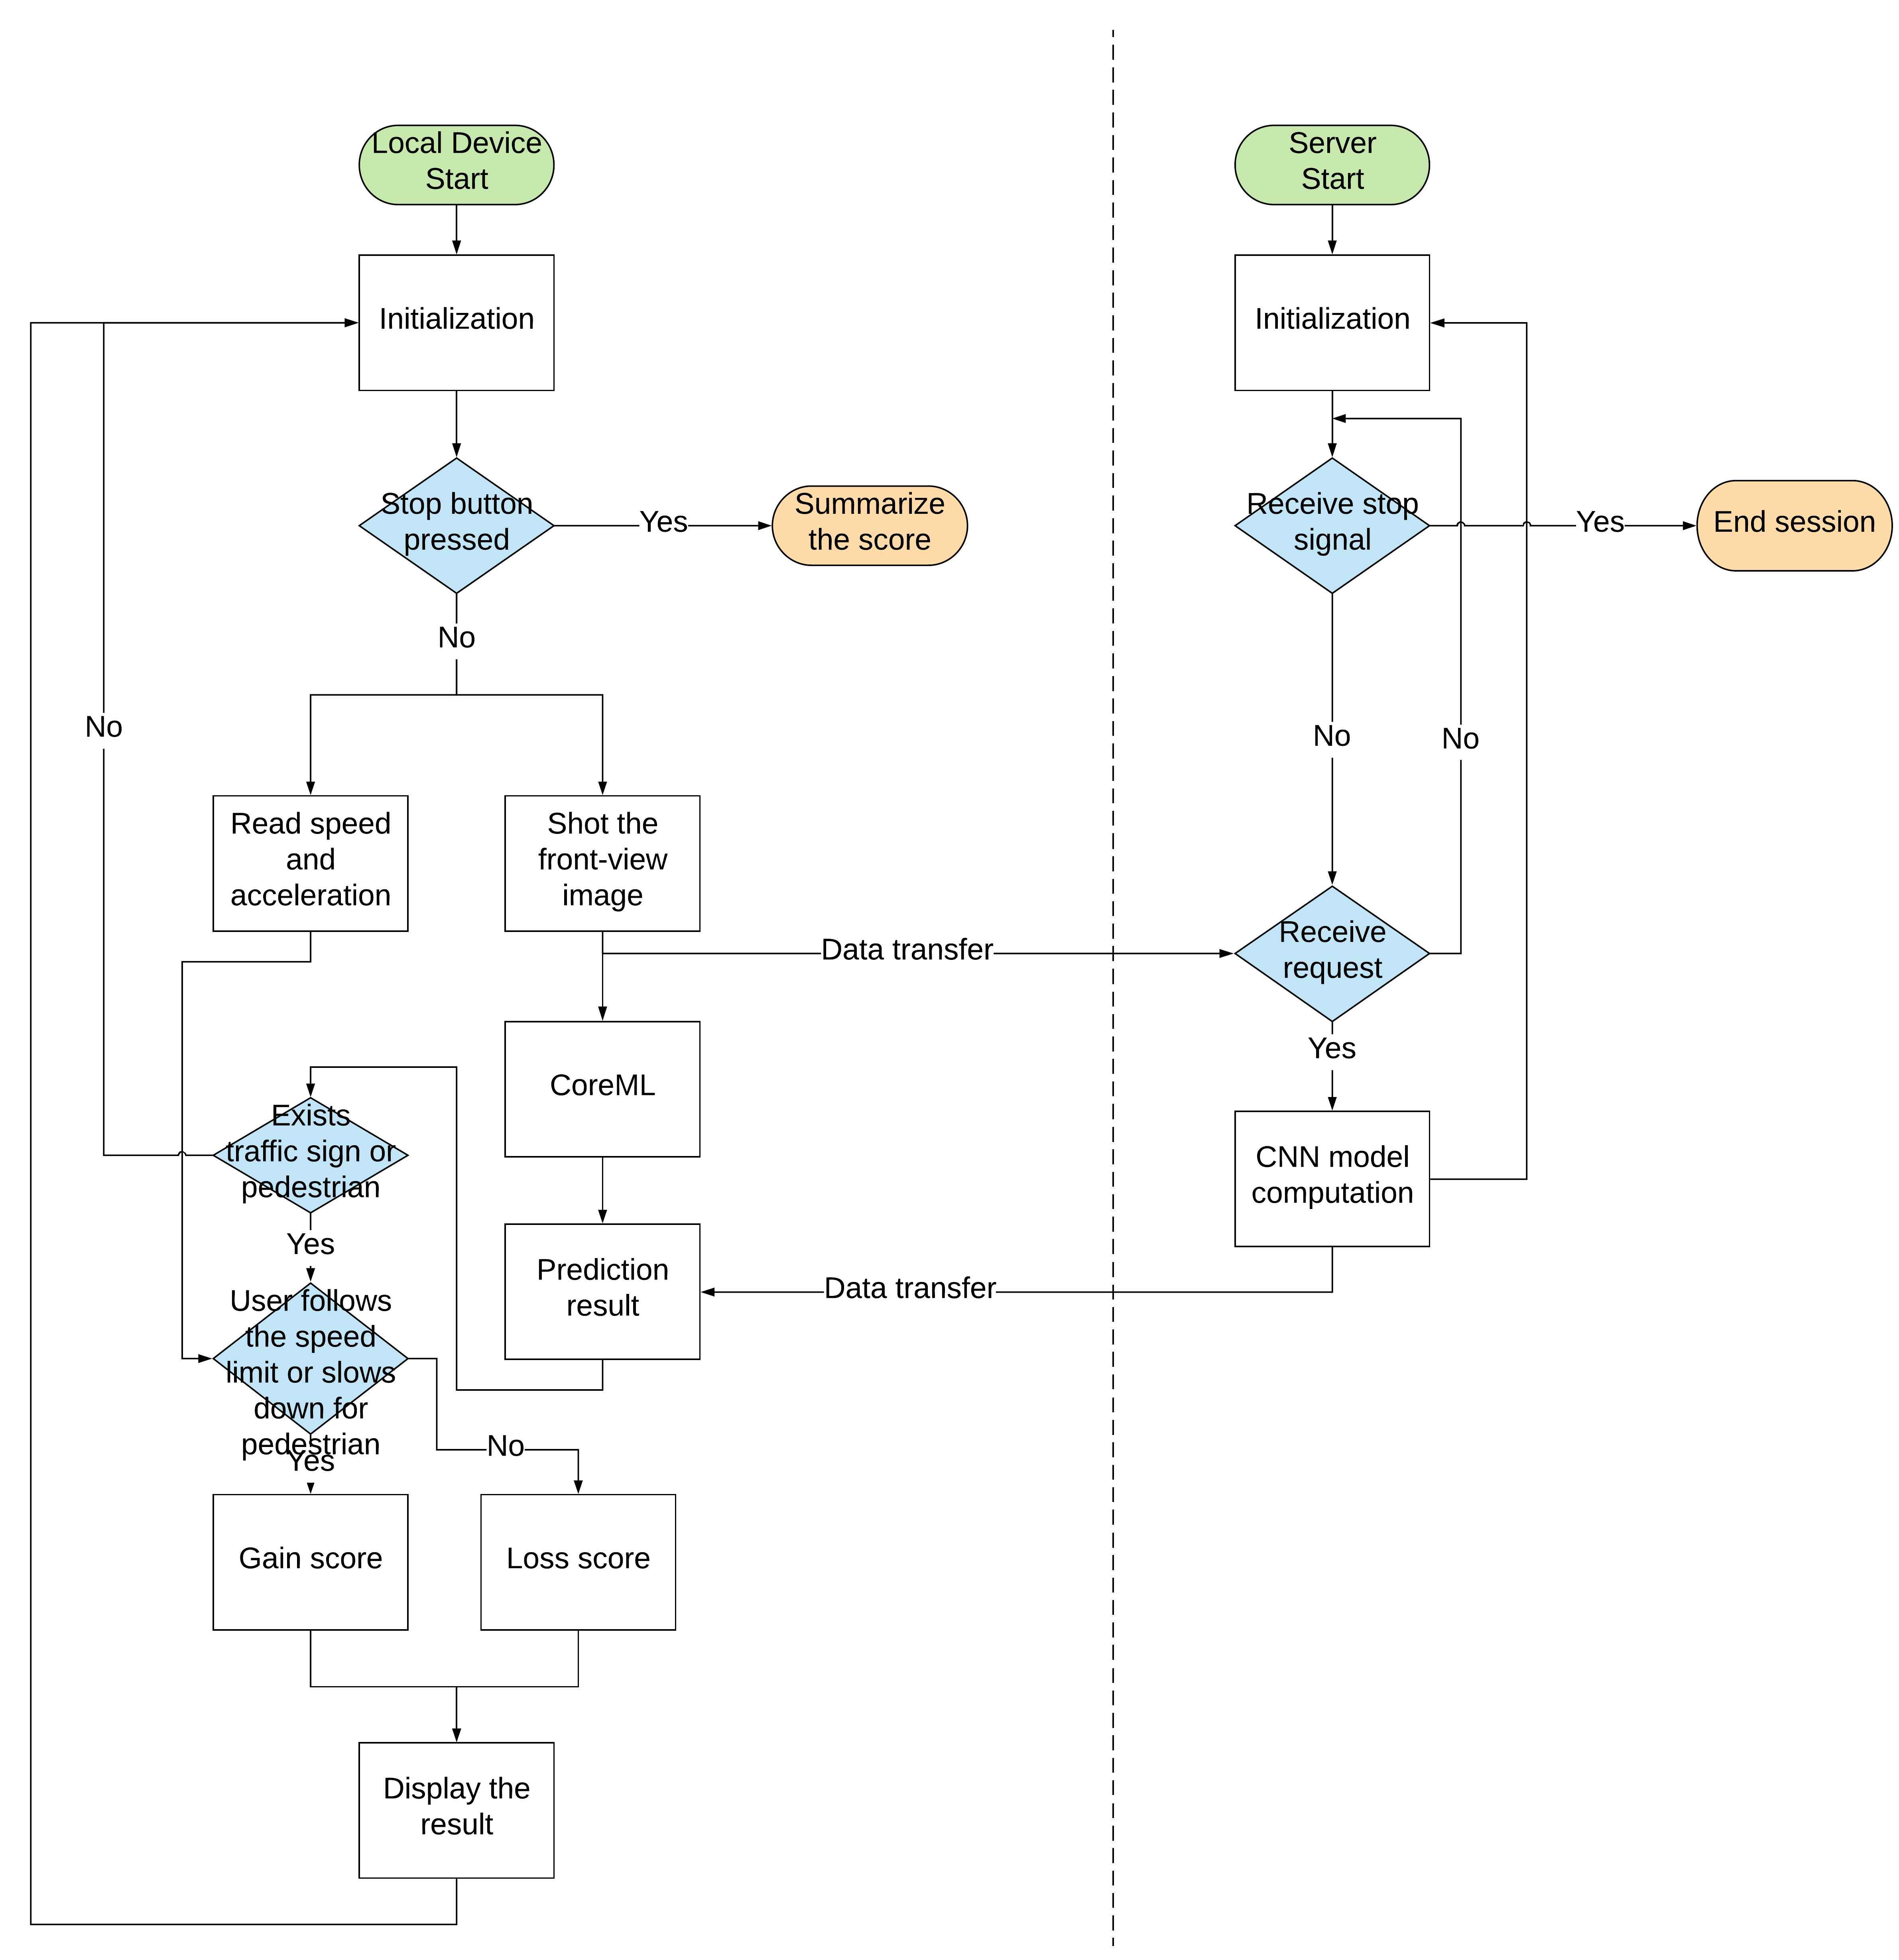
\includegraphics[width=1.2\linewidth]{system_flowchart.png}
    \caption{System Model Flowchart}
    \label{fig:fig_1}
  \end{minipage}
\end{figure}
\subsection{iOS application Design}
We built a simple application with Swift and deploy on iOS 11.2. The application could take the front-view picture periodically, and record both the speed and acceleration at the same time via GPS and accelerometer. The picture will then pass through the trained CNN model (coreML) installed in the bundle, or upload to the cloud service for the prediction. After the translation of the speed limit is done, the application can determine if the user was over speed or not. The illustration of the application design is shown in Figure 2.

\begin{figure}[H]
  \begin{minipage}{.4\textwidth}
    \centering
    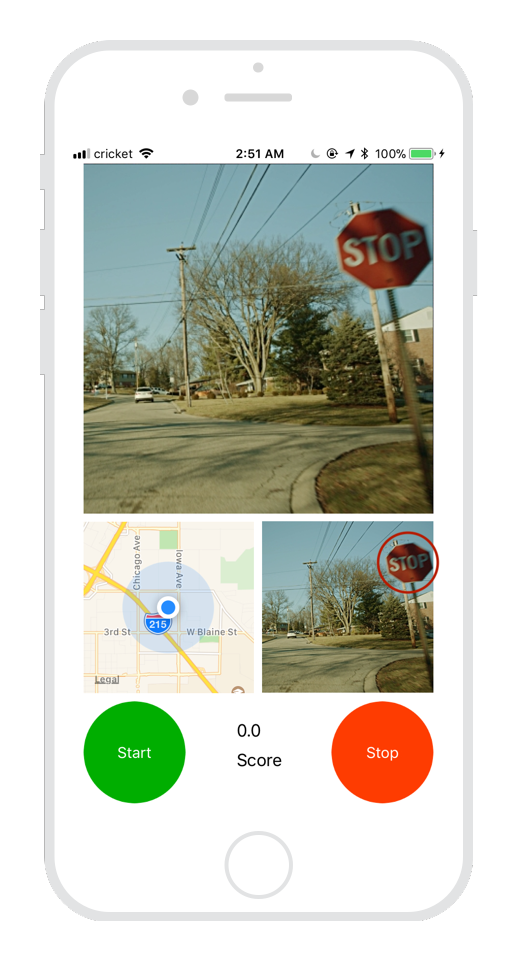
\includegraphics[width=0.6\linewidth]{iOS_design.png}
    \caption{iOS app design}
    \label{fig:fig_1}
  \end{minipage}
\end{figure}

\subsection{Convolutional Neural Network Model}

\subsubsection{Dataset}
There were two popular datasets: GTSRB and LISA dataset. GTSRB contains 43 kinds of different traffic signs in Germany with 39,209 images in the set; LISA traffic sign dataset contains 47 kinds of different US traffic signs with 7,855 annotations on 6,610 frames; LISA traffic light dataset, on the other hand, contains 6 super-classes of traffic lights with total 43,007 frames and 113,888 annotations. Specifically, the images in LISA were taken in South California, which is more close to our proposed scenario.

\subsubsection{Preprocessing}
The training set would first be preprocessed with normalizing, centering and histogram equalizing to help accelerating the train process in the later section. In addition, they would also be augmented, by applying rotation, mirroring and flipping, etc., to mimic more possibilities in the real world cases. And then be separated into training, validating and testing sets. The examples of the common type of sign images in the LISA dataset is shown in Figure 3.

\begin{figure}[H]
\centering
  \begin{minipage}{.4\textwidth}
    \centering
    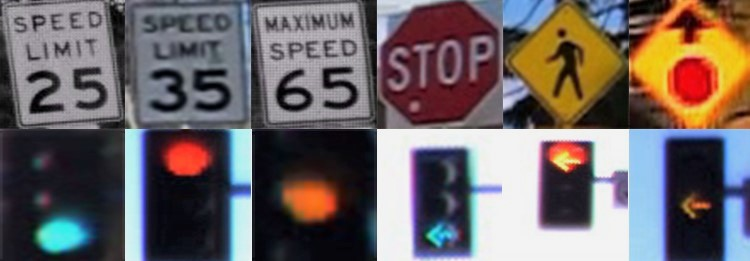
\includegraphics[width=0.8\linewidth]{dataset3.jpg}
    \caption{Example of dataset}
    \label{fig:fig_3}
  \end{minipage}
\end{figure}

\begin{figure}[H]
\begin{center}
\centering
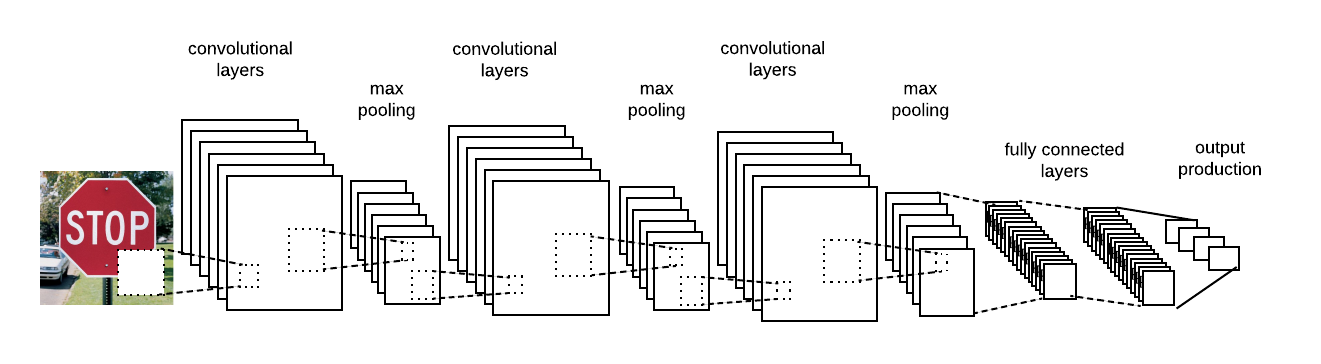
\includegraphics[width=0.9\linewidth]{conv.png}
\caption{Architecture of the proposed CNN model}\end{center}
\label{fig:long}
\end{figure}

\subsubsection{Model Architecture}
In order to do the recognition in our system, we constructed a 6-layer CNN. The model architecture and details of each layer are shown in Figure 4 and Figure 5 respectively. Each convolutional block contains 2 convolutional layers with the same number of kernel and input/output nodes. Additionally, the each block would also followed by a max-pool layer and a drop-out layer. The features extracted by the previously mentioned layers would then be feed to a fully-connected layer with dropout. Finally, the softmax layer would aggregate the result and output the probabilities of the input image with regard to each class.



\begin{figure}[H]
\centering
  \begin{minipage}{.4\textwidth}
    \centering
    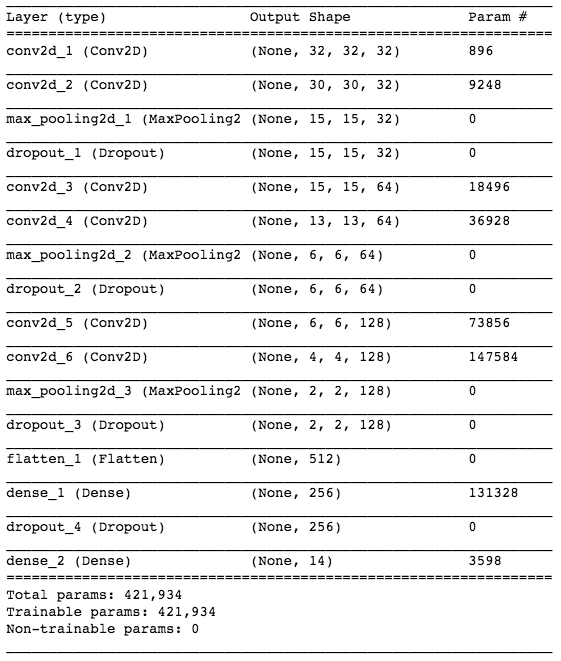
\includegraphics[width=0.8\linewidth]{archi_param.png}
    \caption{CNN layer detail with parameters}
    \label{fig:fig_1}
  \end{minipage}
\end{figure}


\subsection{Cloud Instance Implementation}

Cloud is one of the most important part in our project. However, there are a lot of cloud instances architecture provides by google cloud. In order to get most suitable one for our project. We do some investigation and analysis for the cloud instance implementation.

\begin{table*}
\caption{Cloud instances GPU parameters}
% \centerline { TABLE I  }
% \vskip5pt
% \centerline {Cloud instances GPU parameters}
% \vskip2pt
\centering
\begin{tabular}{|c|c|c|c|c|c|c|}
\hline
\textbf{GPU} & \textbf{Cores} & \textbf{CUDA cores} & \textbf{Frequency} & \textbf{GFLOPs(double)} & \textbf{Memory} & \textbf{Memory bandwidth}\\
\hline
Nvidia Tesla K80 & 2 $\times$ 13(SMX) & 2 $\times$ 2496 & 562MHz & 2 $\times$ 1455 & 2 $\times$ 12GB & 2 $\times$ 240GB/s \\
\hline
Nvidia Tesla P100 & 56(SM) & 3584 & 1126MHz & 4670 & 16GB & 720GB/s\\
\hline
\end{tabular}
\end{table*}

As mentioned above, we use CNN model to recognize traffic signs and traffic lights. While talking about CNN model, it can be run either on CPU and GPU. However, GPU instance is having better performance on running machine learning model. For GPU, the major function decides it needs to do a lot of vector and matrix computation. Those operations are also widely used in machine learning model. Besides, by using GPU, we can do the computation on a large amount of data in higher parallelism. Those make GPU a better choose than CPU to run the machine learning model.   

According to official references, Google cloud provides three different available GPU. They are Nvidia Tesla V100, Nvidia Tesla P100 and Nvidia Tesla K80 respective. However, the Nvidia V100 is for google cloud beta users only. Therefore, we would only do comparison between Nvidia P100 and Nvidia K80.

% The parameters of different kind models are shown below:

% \begin{figure}[hb]
% \centering
%   \begin{minipage}{.4\textwidth}
%     \centering
%     \includegraphics[width=1.0\linewidth]{gpu.jpg}
%     \caption{cloud instances gpu paramrters}
%     \label{fig:fig_1}
%   \end{minipage}
% \end{figure}

% In our project, we are going to choose the generally available GPUs in Google cloud which are NVIDIA Tesla P100 and NVIDIA Tesla K80 instead of using Nivdia V100 which is only for Google cloud beta users. 

Firstly, we show the key hardware differences betweeen Nvidia Tesla P100 and K80 in table I.

In the following part, we are going to focus on memory bandwidth and processing power, which are two key characteristics of GPU relating to machine learning. Besides, we would show the performance of various benchmarks running on different kinds of GPU to verify our analysis. 

\subsubsection{Memory Bandwidth}
Memory bandwidth would be the most important performance metric while running machine learning model on GPU. It shows the ability of GPU to handle large amount of data. The memory bandwidth of different GPU are shown in table II. From the table, we can get that P100 's memory bandwidth is $3 \times$ bigger than K80 per core. 

\begin{table}[H]
% \centerline { TABLE II  }
\caption{Processing power}
\begin{center}
\begin{tabular}{|c|c|}
\hline
\textbf{GPU} & \textbf{\textit{Memory bandwidth}}\\
\hline
Nvidia Tesla K80 & 240GB/s per core \\
\hline
Nvidia Tesla P100 & 720GB/s per core\\
\hline
\end{tabular}
% \label{tab2}
% \setcounter{table}{2}
\end{center}
\end{table}




\subsubsection{Processing Power}
Processing power is also a key characteristic we need to focus on. It indicates the highest speed GPU can achieve to crunch data. It can be presented by the number of CUDA cores multiplies the frequency of the core.
$$Processing \ power = Number \ of \ CUDA \ cores \times frequency $$

The result is shown in table III:

\begin{table}[t]
\caption{Processing power}
\begin{center}
\begin{tabular}{|c|c|c|c|}
\hline
\textbf{GPU} & \textbf{\textit{CUDA cores}}& \textbf{\textit{frequency}}& \textbf{\textit{Processing power}} \\
\hline
Nvidia Tesla K80 & 2496(per core)& 562MHz & 1402752 \\
\hline
Nvidia Tesla P100 & 3584(per core)& 1126MHz & 4035584 \\
\hline
\end{tabular}
\label{tab2}
\end{center}
\end{table}

\subsubsection{Benchmark Result}

In order to make the result more intuitive. We show some evaluation about the influence of running various benchmarks on different kinds of GPUs and CPU below.Those evaluations are gotten from microway.com[5]

The result are shown below:
\begin{figure}[H]
\centering
  \begin{minipage}{.4\textwidth}
    \centering
    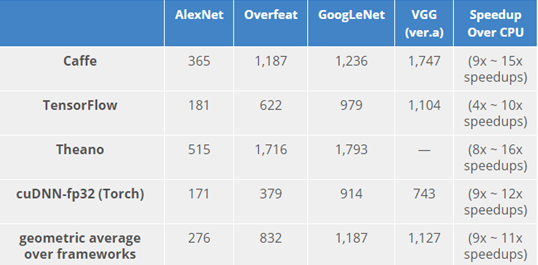
\includegraphics[width=1.0\linewidth]{k80_benchmark.jpg}
    \caption{K80 benchmark result}
    \label{fig:fig_1}
  \end{minipage}
\end{figure}

\begin{figure}[H]
\centering
  \begin{minipage}{.4\textwidth}
    \centering
    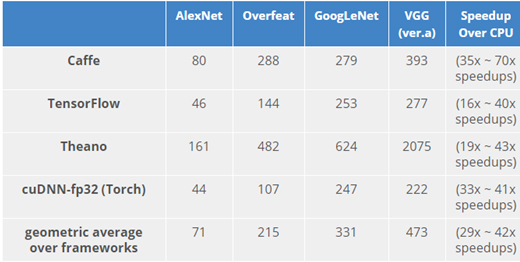
\includegraphics[width=1.0\linewidth]{P100_benchmark.jpg}
    \caption{P100 benchmark result}
    \label{fig:fig_1}
  \end{minipage}
\end{figure}

\begin{figure}[H]
\centering
  \begin{minipage}{.4\textwidth}
    \centering
    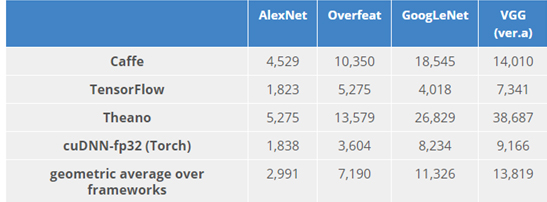
\includegraphics[width=1.0\linewidth]{cpu_only.jpg}
    \caption{CPU only benchmark result}
    \label{fig:fig_1}
  \end{minipage}
\end{figure}

From the experiment, we can get that the speed up over CPU of Nvidia P100 is $4 \times$ higher than speed up over CPU of Nvidia K80 on Tensorflow. 

The comparison above shows the Nvidia Tesla P100 GPU is outperform than Nvidia Tesla K80 from every aspects. 

\section{Evaluation}

\subsection{Experimental setup}

Mobile device, Google cloud instance and terminal machine are used as three platforms we implement our system on. The parameters of them are shown in Table IV.  


\begin{table*}
\caption{Platforms setup}
% \centerline { TABLE B  } 
% \vskip5pt
% \centerline { Platforms setup}
% \vskip2pt
\centering
\begin{tabular}{|c|c|c|c|}
\hline
\textbf{} & \textbf{Google cloud instance }&\textbf{ PC }&
\textbf{Mobile device(Iphone 6s)}\\
\hline
CPU & 2.2GHz Intel Xeon E5 v4(Boardwell) & I5 6400 & 1.85GHz-dual core-64-bit ARMv8-A \\
\hline
Memory & 4.25G & 15G & 2G\\
\hline
GPU & Nvidia Tesla P100   & GTX950 & PowerVR GT7600 \\
\hline
GPU memory bandwidth & 720GB/s & 105GB/s & Unknown \\ 
\hline
CUDA cores/ALU cores & 3584 CUDA cores & 768 CUDA cores & 192 ALU cores \\
\hline
Core frequency & 1126MHz & 1024MHz & Unknown \\
\hline
\end{tabular}
\end{table*}
% \lipsum[2-50]


\subsection{Experiment Evaluation}

\begin{table}[H]
\caption{CNN model test result}
\begin{center}
\begin{tabular}{|c|c|c|}
\hline
\textbf{Dataset} & \textbf{No. of classes}& \textbf{Test accuracy} \\
\hline
GTSRB & 43 & 96.4\% \\
\hline
LISA Traffic Sign & 14 & 99.8\% \\
\hline
LISA Traffic Light& 6 & 99.5\% \\
\hline
\end{tabular}
\label{tab3}
\end{center}
\end{table}

\begin{table}[H]
\caption{CNN model size}
\begin{center}
\begin{tabular}{|c|c|c|}
\hline
\textbf{Model type} & \textbf{Model size} & \textbf{Test accuracy }\\
% & & \textbf{(LISA Traffic Sign test set)}\\
\hline
Keras \textit{(h5)} & 4.51 MB & 99.8\% \\
\hline
coreML \textit{(mlmodel)} & 2.23 MB & 83.2\% \\
\hline
\end{tabular}
\label{tab3}
\end{center}
\end{table}

\subsubsection{CNN model}
The proposed CNN model was already trained by three kinds of datasets with test accuracy shown in Table V. Specifically, since the LISA dataset is a better fit to our proposed scenario, the experiments in the following would focus on LISA rather than GTSRB. In Table VI, we can see that after the conversion of Keras \textit{h5} to coreML \textit{mlmodel}, the size of the model reduced to the half of the origin. Moreover, the test accuracy (using the same test images from LISA Traffic Sign) decreased from 99.8\% to 83.2\%. The result of this experiment shows that the compressing process would affect the accuracy of the model.

\subsubsection{Internet connection}
\begin{table}[H]
\caption{Internet connection}
\begin{center}
\begin{tabular}{|c|c|c|c|}
\hline
& \textbf{Wi-Fi} & \textbf{LTE} & \textbf{4G}\\
\hline
Download & 17.36 Mbps & 7.17 Mbps & 3.92 Mbps\\
\hline
Upload & 11.90 Mbps & 4.20 Mbps & 1.33 Mbps\\
\hline
Ping & 12 ms & 29 ms & 49 ms\\
\hline
\end{tabular}
\label{tab4}
\end{center}
\end{table}
To test the data-transfer time, the test images were all scaled to 32x32 (10 kB). In order to evaluate different kinds of scenario that the driver would encounter while driving, the test image would be uploaded from the smart phone with different Internet connection: Wi-Fi, LTE, and 4G. The download, upload speed with ping time are shown in Table VII. 
\subsubsection{Running time}
The time latency with different platforms and different time-consuming tasks are shown in Figure 9. It's obvious that most of the time are spent in transferring data, which includes the time of uploading the image from mobile device to server and the time of passing the result from server to mobile device. The GCE would need to spend 20 ms to 30 ms for read and preprocess the image and 20 ms to make an inference. The local device averagely uses less than 20 ms for the preproces, and 16 ms for the prediction. On the other hand, It took around 70 ms for the iPhone to make a prediction with coreML.
\subsubsection{Summery}
Generally, if the iPhone was connected to the Internet with LTE steadily, the speed of the inference could reach nearly 4 frames per second with GCE. Meanwhile, it could reach more than 10 frames per second with only coreML model implemented in the application. However, it would trade-off the inference accuracy with the small-size model on the mobile device. Therefore, we think it's better to use the server for inference because the 4-frame-per-second speed is enough for our scenario while the traffic signs would occur in the front view for at least 3 seconds with proper driving speed. If the server took too long with bad Internet connection, the application could still use the inference by the coreML model with lower accuracy after, say, 0.5 second time-out. 
\begin{figure}[H]
\centering
  \begin{minipage}{.4\textwidth}
    \centering
    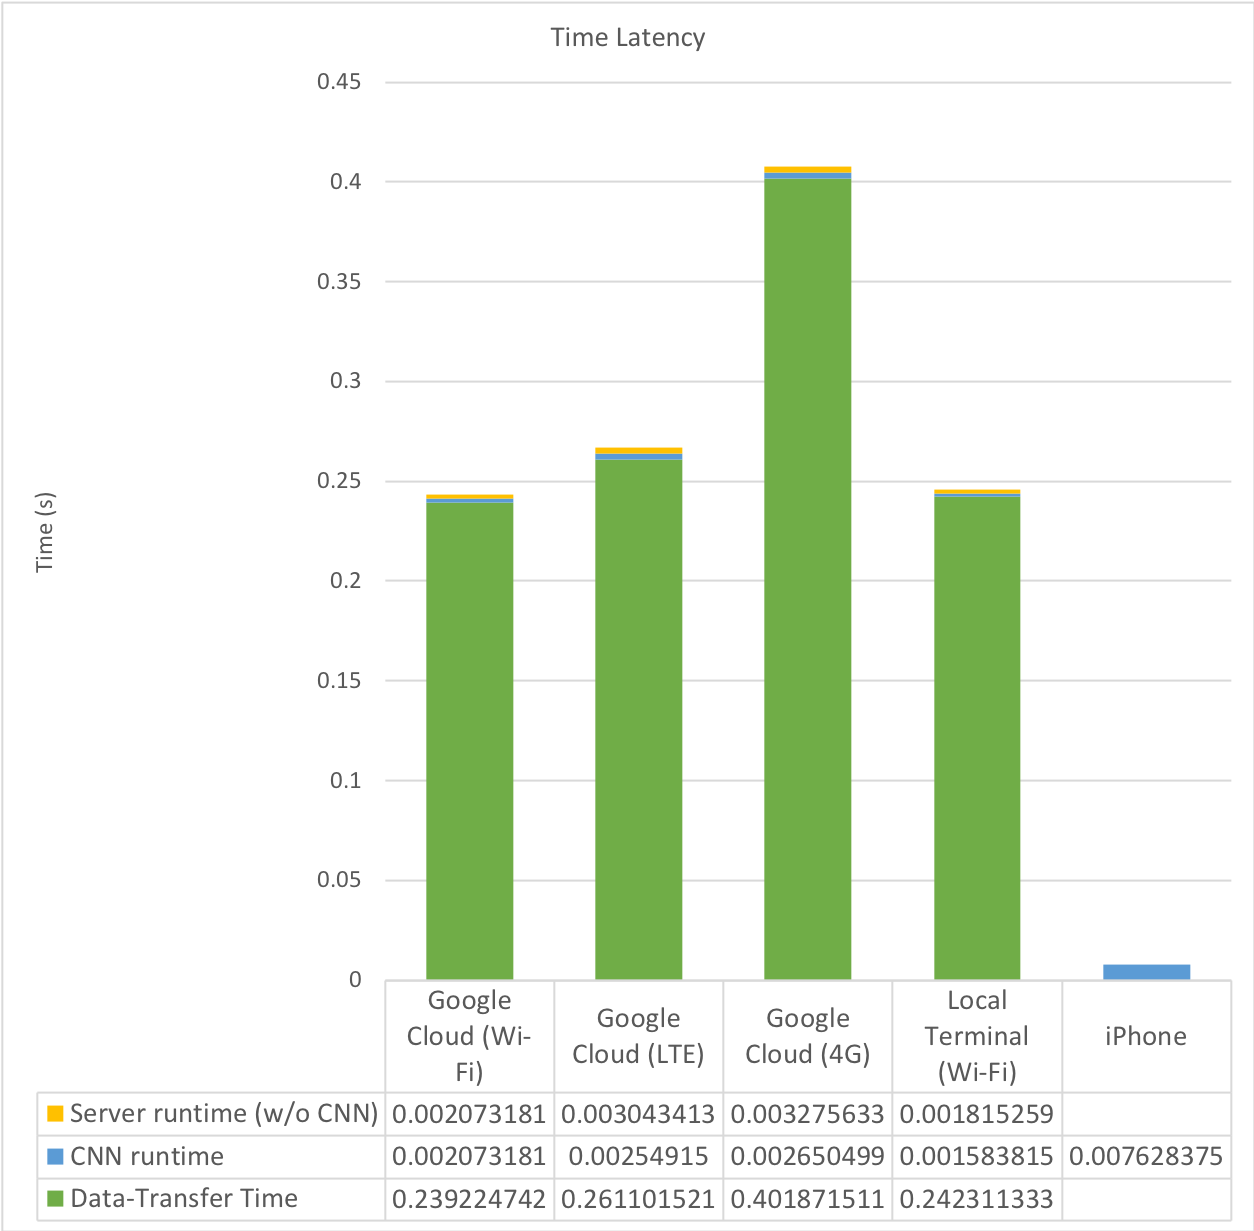
\includegraphics[width=1.0\linewidth]{latency_chart.png}
    \caption{Time latency details}
    \label{fig:fig_1}
  \end{minipage}
\end{figure}



\begin{thebibliography}{00}
\bibitem{b1} Y. Kang, J. Hauswald, C. Gao, A. Rovinski, T. Mudge, J. Mars, L. Tang ``Neurosrgeon:Collaborative Intelligence Between the Cloud and Mobile Edge,'' Processing of the Twenty-second International Conference on Architectural Support for Programming Languages and Operating System. ACM, pp. 615--629, April 2017.
\bibitem{b2} A. Shstanov, P. Yakimov, ``CNN Design For Real-Time Traffic Sign Recognition,''Procedia Engineering, vol.201., 2017, pp. 718--725.
\bibitem{b3} H. Habibi Aghdam, E. Jahani Heravi and D. Puig,``A practical Approach for Detection and Classification of Traffic signs using Convolutional Neural Networks,'' Robotics and Autonomous System, vol. 84., 2016, pp. 97--112.
\bibitem{b4} K. Simonyan, A. Zisserman, ``Very Deep Convolutional Networks for Large-Scale Image Recognition,'' in ARXIV, eprint arXiv:1409.1556, 2014
\bibitem{b6} Microway.com https://www.microway.com/hpc-tech-tips/deep-learning-benchmarks-nvidia-tesla-p100-16gb-pcie-tesla-k80-tesla-m40-gpus/
\end{thebibliography}
\end{document}